\subsection{Caso d'uso UC9: Gestione dei questionari}
\label{UC9}
\begin{figure}[h]
	\centering
	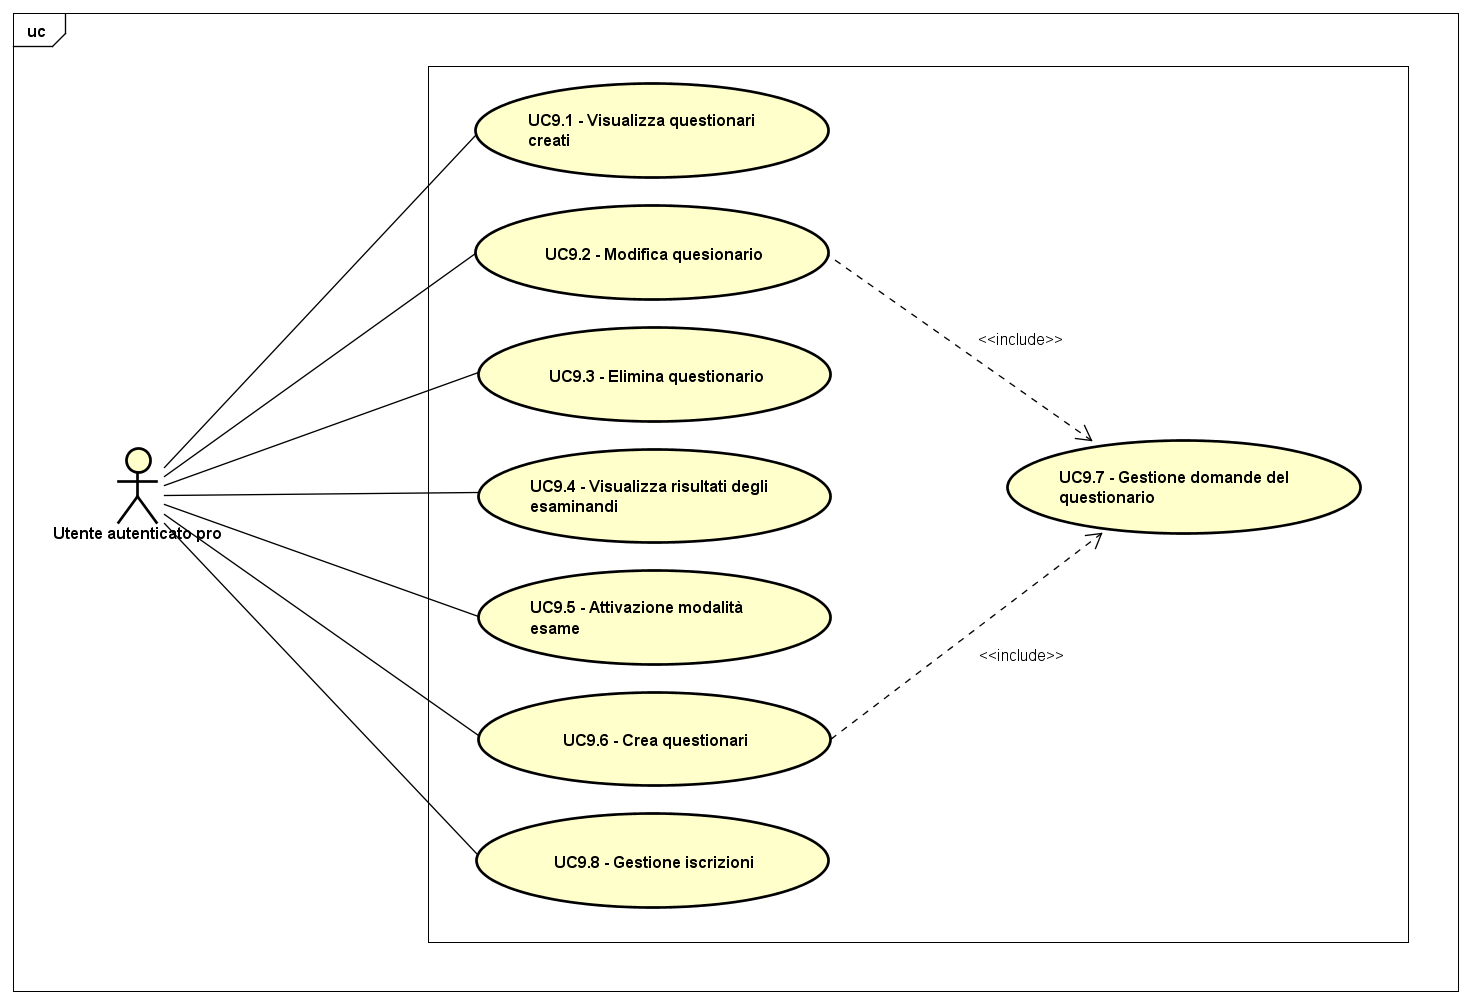
\includegraphics[scale=0.5,keepaspectratio]{UML/UC9.png}
	\caption{UC9: Gestione dei questionari}
\end{figure}
\FloatBarrier
\begin{itemize}
	\item \textbf{Attori}: \uau, \uaupro;
	\item \textbf{Descrizione}: il sistema mostra una schermata in cui l'utente può gestire i propri questionari; 
	\item \textbf{Precondizione}: l'utente accede al sito \textit{web\ped{G}} mediante ad un \textit{browser\ped{G}} supportato dal sistema;
	\item \textbf{Postcondizione}: il sistema ha eseguito le funzionalità scelte dall'utente;
	\item \textbf{Scenario principale}:
		\begin{enumerate}
			\item L'utente può visualizzare i propri questionati (UC9.1);
			\item L'utente può creare nuovi questionari (UC9.2).
		\end{enumerate}
\end{itemize}

	\subsubsection{Caso d'uso UC9.1: Visualizza questionari}
	\label{UC9.1}
	\begin{figure}[h]
		\centering
	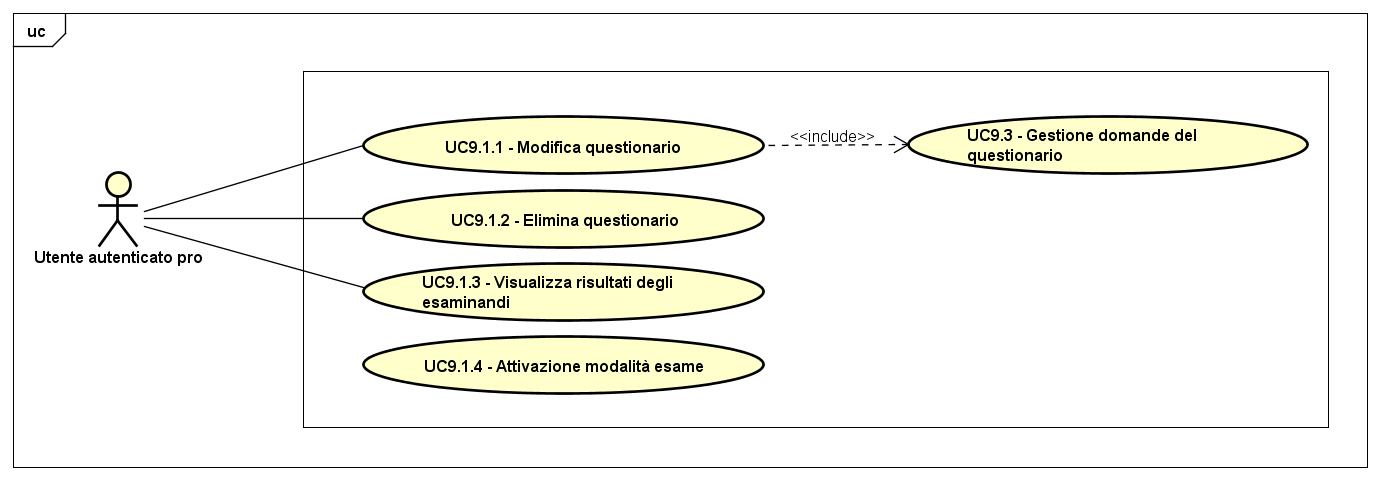
\includegraphics[scale=0.5,keepaspectratio]{UML/UC9_1.png}
		\caption{UC9.1: Visualizza questionari}
	\end{figure}
	\FloatBarrier
	\begin{itemize}
		\item \textbf{Attori}: \uau, \uaupro;
		\item \textbf{Descrizione}: l'utente può visualizzare i propri questionari creati, quelli svolti e quelli salvati per essere eseguiti in un secondo momento; 
		\item \textbf{Precondizione}: l'utente ha selezionato l'opzione "Visualizza questionari" tra le possibilità proposte in UC9;
		\item \textbf{Postcondizione}: il sistema ha mostrato all'utente i questionari e ha permesso delle operazioni su di essi; 
		\item \textbf{Scenario principale}: 
			\begin{enumerate}
				\item L'utente può visualizzare l'elenco dei questionari da svolgere in un secondo momento (UC9.1.1);
				\item L'utente può visualizzare i questionari che ha creato (UC9.1.2); 
				\item L'utente può visualizzare i questionari che ha svolto (UC9.1.3); 
			\end{enumerate}
	\end{itemize}
	
			\subsubsection{Caso d'uso UC9.1.1: Visualizza questionari della lista "Fai più tardi"}
			\label{UC9.1.4}
			\begin{figure}[h]
				\centering
				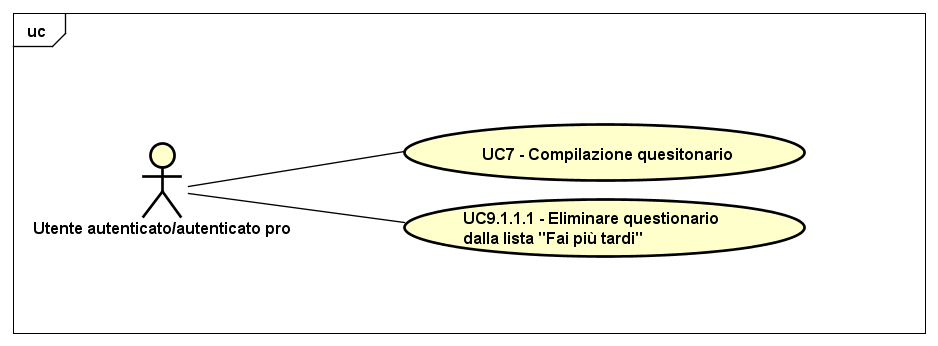
\includegraphics[scale=0.5,keepaspectratio]{UML/UC9_1_1.png}
				\caption{UC9.1.4: Visualizza questionari da svolgere più tardi}
			\end{figure}
			\FloatBarrier
			\begin{itemize}
				\item \textbf{Attori}: \uau, \uaupro;
				\item \textbf{Descrizione}: l'utente può visualizzare l'elenco dei questionari da lui selezionati per essere svolti in un secondo momento;
				\item \textbf{Precondizione}: l'utente ha selezionato l'opzione "Visualizza questionari della lista Fai più tardi" tra le possibilità proposte in UC9.1;
				\item \textbf{Postcondizione}: il sistema ha eseguito le opzioni scelte dall'utente;
				\item \textbf{Scenario principale}: 
				\begin{enumerate}
					\item L'utente può compilare il questionario (UC7);
					\item L'utente può eliminare un questionario dalla lista "Fai più tardi" (UC9.1.1.1).
				\end{enumerate}
			\end{itemize}
				
				\subsubsection{Caso d'uso UC9.1.1.1: Eliminare questionario dalla lista "Fai più tardi"}
				\label{UC9.1.4.1}
				\begin{figure}[h]
					\centering
					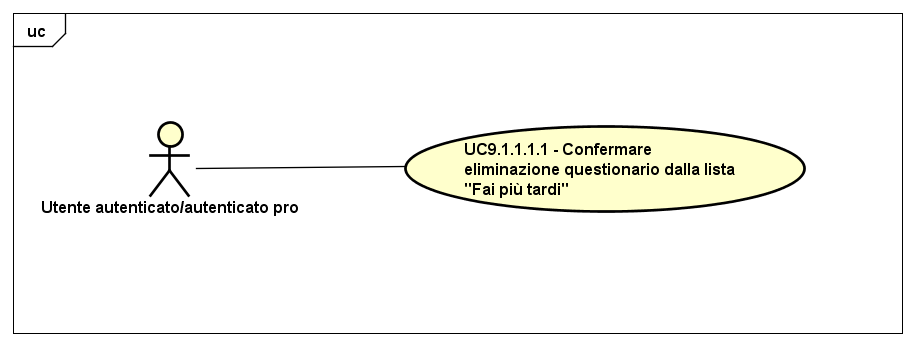
\includegraphics[scale=0.5,keepaspectratio]{UML/UC9_1_1_1.png}
					\caption{UC9.1.1.1: Eliminare questionario dalla lista "Fai più tardi"}
				\end{figure}
				\FloatBarrier
				\begin{itemize}
					\item \textbf{Attori}: \uau, \uaupro;
					\item \textbf{Descrizione}: l'utente ha la possibilità di eliminare il questionario selezionato dalla lista "Fai più tardi";
					\item \textbf{Precondizione}: l'utente ha selezionato l'opzione "Eliminare questionario dalla lista Fai più tardi" tra le possibilità proposte in UC9.1.1 su un questionario;
					\item \textbf{Postcondizione}: il sistema ha eliminato, dall'elenco dei questionari da svolgere più tardi, quello selezionato;
					\item \textbf{Scenario principale}: l'utente può confermare l'eliminazione del questionario dall'elenco dei questionari da svolgere più tardi (UC9.1.1.1.1).	
				\end{itemize}
				
					\subsubsection{Caso d'uso UC9.1.1.1.1: Confermare eliminazione questionario dalla lista "Fai più tardi"}
					\label{UC9.1.1.1.1}
					\begin{itemize}
						\item \textbf{Attori}: \uau, \uaupro;
						\item \textbf{Descrizione}: l'utente dopo aver scelto di eliminare il questionario deve confermare tale operazione;
						\item \textbf{Precondizione}: l'utente ha scelto di eliminare il questionario;
						\item \textbf{Postcondizione}: l'utente ha eliminato il questionario;
						\item \textbf{Scenario principale}: l'utente deve confermare l'eliminazione del questionario dalla lista "Fai più tardi". Una volta fatto ciò viene mandato nella pagina che contiene la lista dei questionari "Fai più tardi" (UC9.1.1);
						\item \textbf{Scenari alternativi}: L'utente non conferma l'eliminazione del questionario dalla lista "Fai più tardi" e viene mandato alla schermata precedente.
					\end{itemize}
							
		\subsubsection{Caso d'uso UC9.1.2: Visualizza questionari creati}
		\label{UC9.1.2}
		\begin{figure}[h]
			\centering
		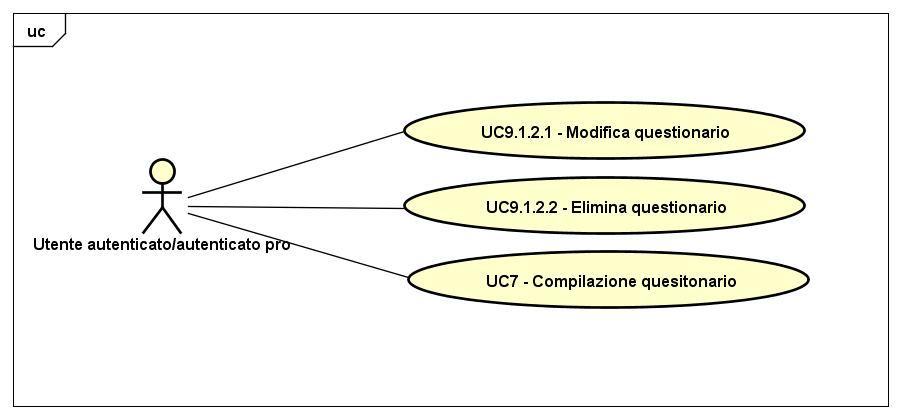
\includegraphics[scale=0.5,keepaspectratio]{UML/UC9_1_2.png}
			\caption{UC9.1.2: Visualizza questionari creati}
		\end{figure}
		\FloatBarrier
		\begin{itemize}
			\item \textbf{Attori}: \uau, \uaupro;
			\item \textbf{Descrizione}: l'utente può visualizzare i questionari da lui creati;
			\item \textbf{Precondizione}: l'utente ha selezionato l'opzione "Visualizza questionari creati" tra le possibilità proposte in UC9.1;
			\item \textbf{Postcondizione}: il sistema ha eseguito le opzioni scelte dall'utente;
			\item \textbf{Scenario principale}: 
				\begin{enumerate}
					\item L'utente può modificare un questionario creato (UC9.1.2.1);
					\item L'utente può eliminare un questionario creato (UC9.1.2.2);
					\item L'utente può compilare un questionario (UC7).
				\end{enumerate}
		\end{itemize}
		
			\subsubsection{Caso d'uso UC9.1.2.1: Modifica questionario}
			\label{UC9.1.2.1}
			\begin{figure}[h]
				\centering
			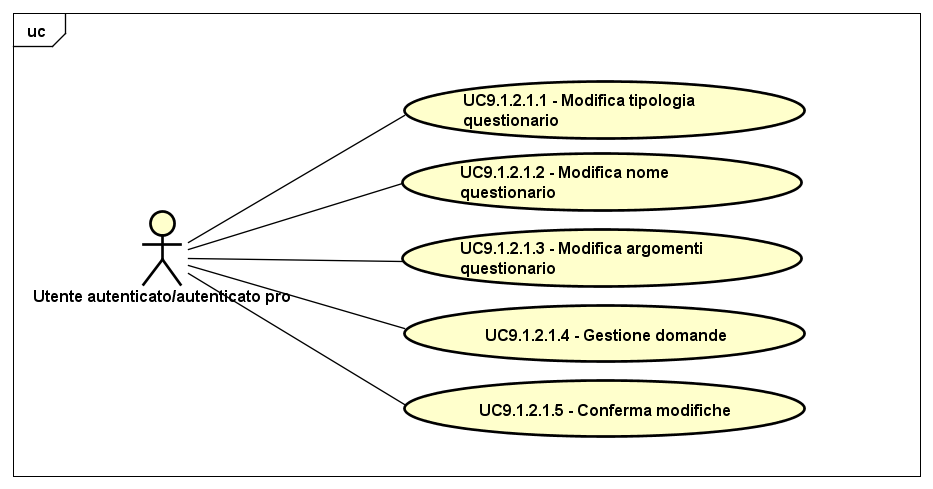
\includegraphics[scale=0.5,keepaspectratio]{UML/UC9_1_2_1.png}
				\caption{UC9.1.2.1: Modifica questionario}
			\end{figure}
			\FloatBarrier
			\begin{itemize}
				\item \textbf{Attori}: \uau, \uaupro;
				\item \textbf{Descrizione}: l'utente può modificare il questionario selezionato;
				\item \textbf{Precondizione}: l'utente ha selezionato l'opzione "Modifica questionario" tra le possibilità proposte in UC9.1.2 su un questionario;
				\item \textbf{Postcondizione}: l'utente ha modificato il questionario selezionato; 
				\item \textbf{Scenario principale}:
					\begin{enumerate}
						\item L'utente può modificare la tipologia del questionario (UC9.1.2.1.1);
						\item L'utente può modificare il nome del questionario (UC9.1.2.1.2);
						\item L'utente può modificare gli argomenti del questionario (UC9.1.2.1.3);
						\item L'utente può gestire le domande del questionario (UC9.1.2.1.4);
						\item L'utente può confermare le modifiche fatte (UC9.1.2.1.5).
					\end{enumerate}
			\end{itemize}
			
					\subsubsection{Caso d'uso UC9.1.2.1.1: Modifica tipologia questionario}
					\label{UC9.1.2.1.1}
					\begin{itemize}
						\item \textbf{Attori}: \uau, \uaupro;
						\item \textbf{Descrizione}: l'utente può modificare la tipologia del questionario facendolo passare da pubblico a privato e viceversa; 
						\item \textbf{Precondizione}: l'utente ha selezionato l'opzione "Modifica tipologia questionario" tra le scelte possibili in UC9.1.2.1;
						\item \textbf{Postcondizione}: l'utente ha modificato la tipologia del questionario;
						\item \textbf{Scenario principale}: l'utente modifica la tipologia del questionario;
						\item \textbf{Scenari alternativi}: l'utente non possiede un account pro e tenta di selezionare la tipologia privata per il questionario. Viene mandato in una pagina in cui può cambiare la tipologia del proprio account (UC5.7); 
					\end{itemize}
											
					\subsubsection{Caso d'uso UC9.1.2.1.2: Modifica nome questionario}
					\label{UC9.1.2.1.2}
					\begin{itemize}
						\item \textbf{Attori}: \uau, \uaupro;
						\item \textbf{Descrizione}: l'utente può modificare il nome del questionario; 
						\item \textbf{Precondizione}: l'utente ha selezionato l'opzione "Modifica nome questionario" tra le scelte possibili in UC9.1.2.1;
						\item \textbf{Postcondizione}: l'utente ha modificato il nome del questionario; 
						\item \textbf{Scenario principale}: l'utente modifica il nome del questionario;
					\end{itemize}
					
					\subsubsection{Caso d'uso UC9.1.2.1.3: Modifica argomenti questionario}
					\label{UC9.1.2.1.3}
					\begin{figure}[h]
						\centering
					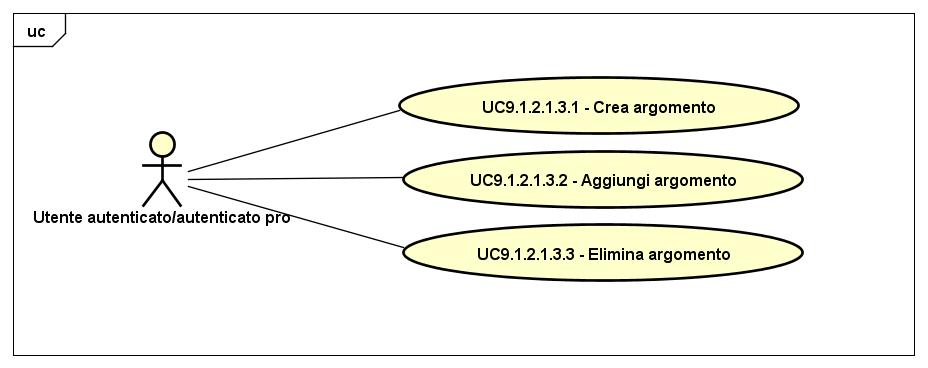
\includegraphics[scale=0.5,keepaspectratio]{UML/UC9_1_2_1_3.png}
						\caption{UC9.1.2.1.3: Modifica argomenti questionario}
					\end{figure}
					\FloatBarrier
					\begin{itemize}
						\item \textbf{Attori}: \uau, \uaupro;
						\item \textbf{Descrizione}: l'utente può decidere di modificare gli argomenti che riassumono il questionario, aggiungendone oppure togliendone qualcuno; 
						\item \textbf{Precondizione}: l'utente ha selezionato l'opzione "Modifica argomenti questionario" tra le scelte possibili in UC9.1.2.1; 
						\item \textbf{Postcondizione}: l'utente ha modificato gli argomenti che riassumono il questionario; 
						\item \textbf{Scenario principale}:
							\begin{enumerate}
								\item L'utente può creare un nuovo argomento (UC9.1.2.1.3.1);
								\item L'utente può aggiungere un nuovo argomento all'elenco di argomenti (UC9.1.2.1.3.2);
								\item L'utente può eliminare un argomento (UC9.1.2.1.3.3);
							\end{enumerate}
						\item \textbf{Scenari alternativi}: l'utente elimina tutti gli argomenti. In questo caso deve inserirne almeno uno e viene mandato al caso d'uso UC9.1.2.1.3.2.
					\end{itemize}
					
						\subsubsection{Caso d'uso UC9.1.2.1.3.1: Crea argomento}
						\label{UC9.1.2.1.3.1}
						\begin{figure}[h]
							\centering
						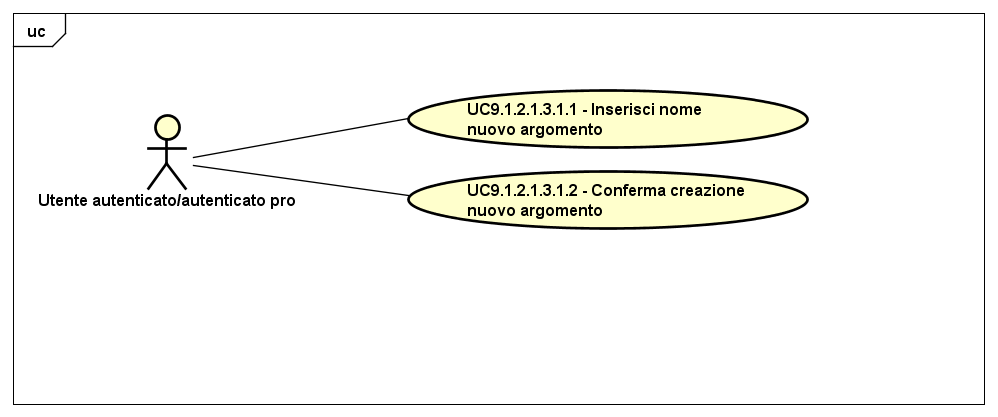
\includegraphics[scale=0.5,keepaspectratio]{UML/UC9_1_2_1_3_1.png}
							\caption{UC9.1.2.1.3.1: Crea argomento}
						\end{figure}
						\FloatBarrier
						\begin{itemize}
							\item \textbf{Attori}: \uau, \uaupro;
							\item \textbf{Descrizione}: l'utente può creare un nuovo argomento non presente tra quelli già esistenti;
							\item \textbf{Precondizione}: l'utente ha selezionato l'opzione "Crea argomento" tra le scelte possibili;
							\item \textbf{Postcondizione}: l'utente ha creato un nuovo argomento; 
							\item \textbf{Scenario principale}:
								\begin{enumerate}
									\item L'utente deve inserire il nome del nuovo argomento (UC9.1.2.1.3.1.1);
									\item L'utente deve confermare il nuovo argomento (UC9.1.2.1.3.1.2).
								\end{enumerate}
						\end{itemize}
						
							\subsubsection{Caso d'uso UC9.1.2.1.3.1.1: Inserisci nome nuovo argomento}
							\label{UC9.1.2.1.3.1.1}
							\begin{itemize}
								\item \textbf{Attori}: \uau, \uaupro;
								\item \textbf{Descrizione}: l'utente inserisce il nome del nuovo argomento;
								\item \textbf{Precondizione}: l'utente ha selezionato l'opzione "Inserisci nome utente" tra le scelte possibili in UC9.1.2.1.3.1;
								\item \textbf{Postcondizione}: l'utente ha inserito il nome del nuovo argomento;
								\item \textbf{Scenario principale}: l'utente inserisce il nome del nuovo argomento;
							\end{itemize}
							
							\subsubsection{Caso d'uso UC9.1.2.1.3.1.2: Conferma creazione nuovo argomento}
							\label{UC9.1.2.1.3.1.2}
							\begin{itemize}
								\item \textbf{Attori}: \uau, \uaupro;
								\item \textbf{Descrizione}: l'utente conferma il nuovo argomento;
								\item \textbf{Precondizione}: l'utente ha selezionato l'opzione "Conferma creazione nuovo argomento" tra le scelte possibili in UC9.1.2.1.3.1;
								\item \textbf{Postcondizione}: l'utente ha confermato la creazione di un nuovo argomento;
								\item \textbf{Scenario principale}: l'utente conferma la creazione di un nuovo argomento;
								\item \textbf{Scenari alternativi}: 
									\begin{enumerate}
										\item L'utente seleziona un nome che già esiste. Viene riportato alla situazione del caso d'uso UC9.1.2.1.3.1.1;
										\item L'utente annulla l'operazione e viene portato alla situazione del caso d'uso UC9.1.2.1.3;
									\end{enumerate}
						
							\end{itemize}
						
						\subsubsection{Caso d'uso UC9.1.2.1.3.2: Aggiungi argomento}
						\label{UC9.1.2.1.3.2}
						\begin{figure}[h]
							\centering
							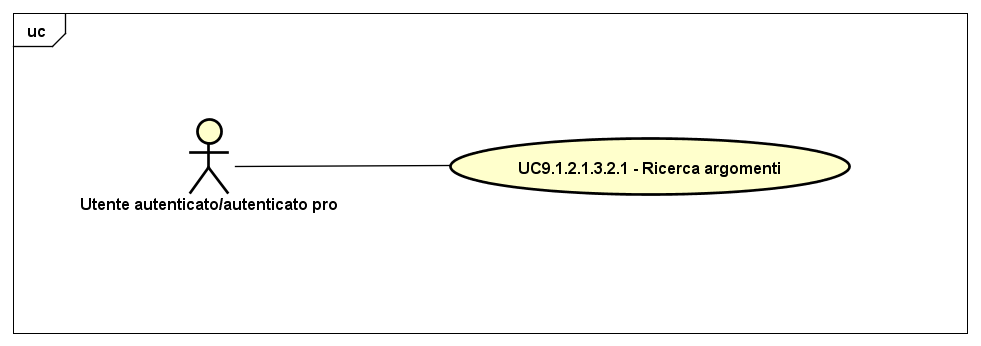
\includegraphics[scale=0.5,keepaspectratio]{UML/UC9_1_2_1_3_2.png}
							\caption{UC9.1.2.1.3.2: Aggiungi argomento}
						\end{figure}
						\FloatBarrier
						\begin{itemize}
							\item \textbf{Attori}: \uau, \uaupro;
							\item \textbf{Descrizione}: l'utente può aggiungere altri argomenti selezionandoli tra quelli archiviati;  
							\item \textbf{Precondizione}: l'utente ha selezionato l'opzione "Aggiungi argomento" tra le scelte possibili;
							\item \textbf{Postcondizione}: l'utente ha selezionato dei nuovi argomenti;
							\item \textbf{Scenario principale}: l'utente può ricercare argomenti tra quelli archiviati (UC9.1.2.1.3.2.1);
						\end{itemize}
						
							\subsubsection{Caso d'uso UC9.1.2.1.3.2.1: Ricerca argomenti}
							\label{UC9.1.2.1.3.2.1}
							\begin{figure}[h]
								\centering
								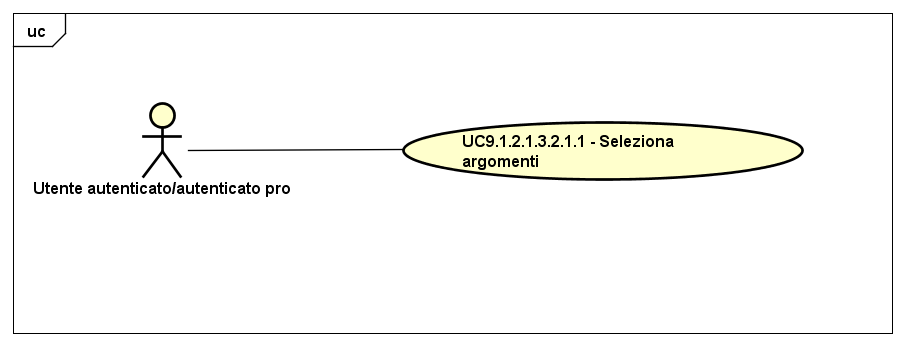
\includegraphics[scale=0.5,keepaspectratio]{UML/UC9_1_2_1_3_2_1.png}
								\caption{UC9.1.2.1.3.2: Aggiungi argomento}
							\end{figure}
							\FloatBarrier
							\begin{itemize}
								\item \textbf{Attori}: \uau, \uaupro;
								\item \textbf{Descrizione}: l'utente può eseguire una ricerca tra gli argomenti archiviati; 
								\item \textbf{Precondizione}: l'utente ha selezionato l'opzione "Ricerca argomenti" tra le scelte possibili in UC9.1.2.1.3.2;
								\item \textbf{Postcondizione}: l'utente ha ricercato tra gli argomenti archiviati;
								\item \textbf{Scenario principale}: l'utente può selezionare gli argomenti (UC9.1.2.1.3.2.1.1); 
								\item \textbf{Scenari alternativi}: nel caso in cui non ci sia nessun risultato dalla ricerca all'utente viene proposta la possibilità di creare un nuovo argomento (UC9.1.2.1.3.1);
							\end{itemize}
							
								\subsubsection{Caso d'uso UC9.1.2.1.3.2.1.1: Seleziona argomenti}
								\label{UC9.1.2.1.3.2.2}
								\begin{itemize}
									\item \textbf{Attori}: \uau, \uaupro;
									\item \textbf{Descrizione}: l'utente può selezionare gli argomenti tra quelli ottenuti dalla ricerca;
									\item \textbf{Precondizione}: l'utente ha ottenuto una lista di risultati;
									\item \textbf{Postcondizione}: l'utente ha selezionato degli argomenti; 
									\item \textbf{Scenario principale}: l'utente seleziona gli argomenti;
								\end{itemize}
						
						\subsubsection{Caso d'uso UC9.1.2.1.3.3: Elimina argomento}
						\label{UC9.1.2.1.3.3}
						\begin{figure}[h]
							\centering
							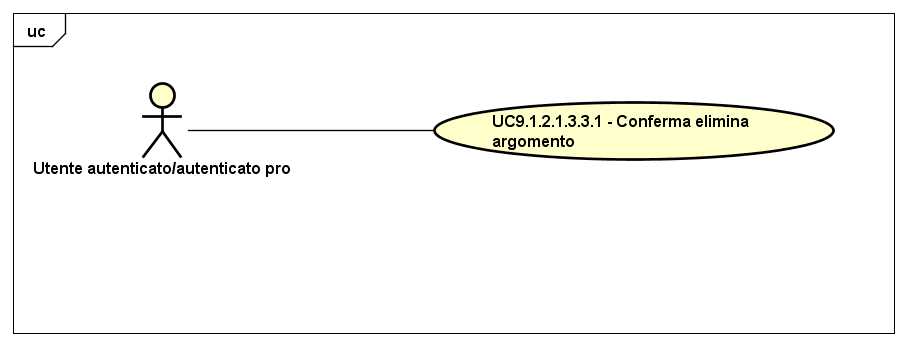
\includegraphics[scale=0.5,keepaspectratio]{UML/UC9_1_2_1_3_3.png}
							\caption{UC9.1.2.1.3.3: Elimina argomento}
						\end{figure}
						\FloatBarrier
						\begin{itemize}
							\item \textbf{Attori}: \uau, \uaupro;
							\item \textbf{Descrizione}: l'utente può eliminare un argomento da un questionario;
							\item \textbf{Precondizione}: l'utente ha selezionato l'opzione "Elimina argomento" tra le scelte possibili;
							\item \textbf{Postcondizione}: l'utente ha eliminato un argomento;
							\item \textbf{Scenario principale}: l'utente deve confermare di voler eliminare l'argomento (UC9.1.2.1.3.3.1); 
							\item \textbf{Scenari alternativi}: l'utente ha cancellato tutti gli argomenti. Deve allora inserirne almeno uno, viene allora rimandato a UC9.1.2.1.3.2.
						\end{itemize}
						
							\subsubsection{Caso d'uso UC9.1.2.1.3.3.1: Conferma elimina argomento}
							\label{UC9.1.2.1.3.3.1}
							\begin{itemize}
								\item \textbf{Attori}: \uau, \uaupro;
								\item \textbf{Descrizione}: l'utente deve confermare di voler eliminare l'argomento;
								\item \textbf{Precondizione}: l'utente ha deciso di voler eliminare l'argomento;
								\item \textbf{Postcondizione}: l'utente ha eliminato un argomento;
								\item \textbf{Scenario principale}: l'utente conferma di voler eliminare l'argomento. 
								\item \textbf{Scenari alternativi}: l'utente annulla l'eliminazione dell'argomento, viene allora rimandato a UC9.1.2.1.3.
							\end{itemize}						
						
					\subsubsection{Caso d'uso UC9.1.2.1.4: Gestione domande}
					\label{UC9.1.2.1.4}
					\begin{figure}[h]
						\centering
					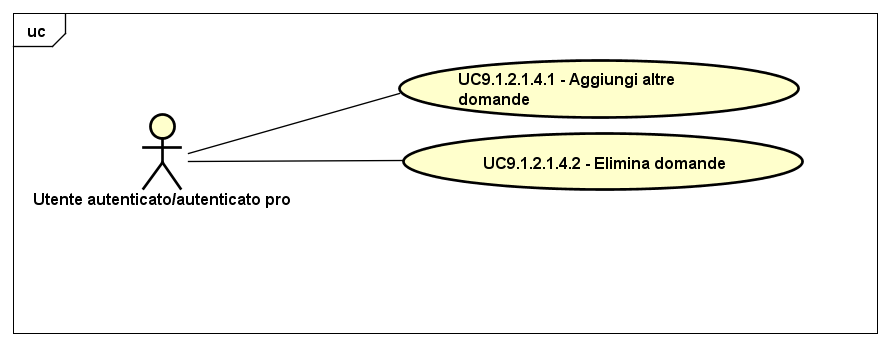
\includegraphics[scale=0.5,keepaspectratio]{UML/UC9_1_2_1_4.png}
						\caption{UC9.1.2.1.4: Gestione domande}
					\end{figure}
					\FloatBarrier
					\begin{itemize}
						\item \textbf{Attori}: \uau, \uaupro;
						\item \textbf{Descrizione}: l'utente può gestire le domande di un proprio questionario, aggiungendone oppure togliendone;
						\item \textbf{Precondizione}: l'utente ha selezionato l'opzione "Gestione domande" tra le scelte possibili in UC9.1.2.1.4;
						\item \textbf{Postcondizione}: l'utente ha gestito le domande di un questionario;
						\item \textbf{Scenario principale}: 
							\begin{enumerate}
								\item L'utente aggiunge altre domande (UC9.1.2.1.4.1);
								\item L'utente elimina una domanda (UC9.1.2.1.4.2).
							\end{enumerate}
					\end{itemize}
					
						\subsubsection{Caso d'uso UC9.1.2.1.4.1: Aggiungi altre domande}
						\label{UC9.1.2.1.4.1}
						\begin{figure}[h]
							\centering
						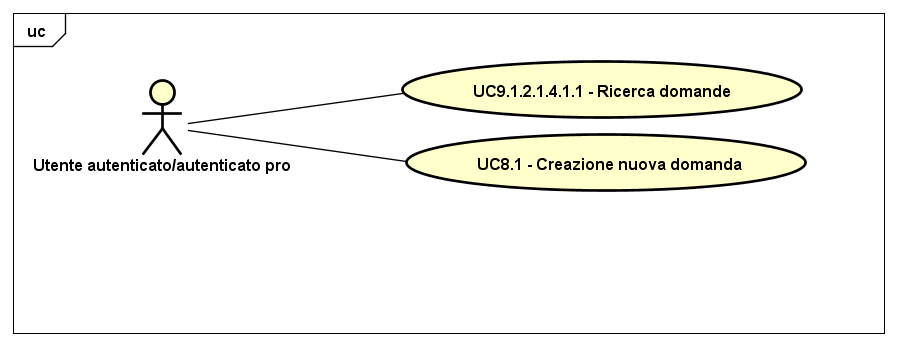
\includegraphics[scale=0.5,keepaspectratio]{UML/UC9_1_2_1_4_1.png}
							\caption{UC9.1.2.1.4.1: Aggiungi altre domande}
						\end{figure}
						\FloatBarrier
						\begin{itemize}
							\item \textbf{Attori}: \uau, \uaupro;
							\item \textbf{Descrizione}: l'utente può aggiungere altre domande cercando tra quelle già memorizzate nell'archivio oppure creandone una nuova; 
							\item \textbf{Precondizione}: l'utente ha selezionato l'opzione "Aggiungi altre domande" tra le scelte possibili in UC9.1.2.1.4;
							\item \textbf{Postcondizione}: l'utente ha aggiunto nuove domande;
							\item \textbf{Scenario principale}:
								\begin{enumerate}
									\item L'utente può eseguire una ricerca nelle domande archiviate (UC9.1.2.1.4.1.1);
									\item L'utente può creare una nuova domanda (UC8.1);
								\end{enumerate}
						\end{itemize}
						
							\subsubsection{Caso d'uso UC9.1.2.1.4.1.1: Ricerca domande}
							\label{UC9.1.2.1.4.1.1}
							\begin{figure}[h]
								\centering
								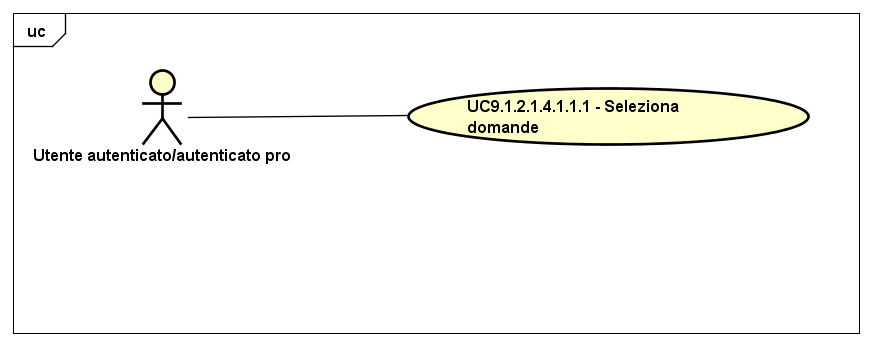
\includegraphics[scale=0.5,keepaspectratio]{UML/UC9_1_2_1_4_1_1.png}
								\caption{UC9.1.2.1.4.1.1: Ricerca domande}
							\end{figure}
							\FloatBarrier
							\begin{itemize}
								\item \textbf{Attori}: \uau, \uaupro;
								\item \textbf{Descrizione}: l'utente può eseguire una ricerca tra le domande archiviate; 
								\item \textbf{Precondizione}: l'utente ha selezionato l'opzione "Ricerca domande" tra le scelte possibili in UC9.1.2.1.4.1;
								\item \textbf{Postcondizione}: l'utente ha ricercato tra le domande archiviate;
								\item \textbf{Scenario principale}: l'utente può selezionare le domande (UC9.1.2.1.4.1.1.1); 
								\item \textbf{Scenari alternativi}: nel caso in cui non ci sia nessun risultato dalla ricerca all'utente viene proposta la possibilità di creare una nuova domanda (UC8.1);
							\end{itemize}
							
								\subsubsection{Caso d'uso UC9.1.2.1.4.1.1.1: Seleziona domande}
								\label{UC9.1.2.1.4.1.1.1}
								\begin{itemize}
									\item \textbf{Attori}: \uau, \uaupro;
									\item \textbf{Descrizione}: l'utente può selezionare le domande tra quelle ottenute dalla ricerca;
									\item \textbf{Precondizione}: l'utente ha ottenuto una lista di risultati;
									\item \textbf{Postcondizione}: l'utente ha selezionato delle domande; 
									\item \textbf{Scenario principale}: l'utente seleziona le domande;
								\end{itemize}
							
						\subsubsection{Caso d'uso UC9.1.2.1.4.2: Elimina domanda}
						\label{UC9.1.2.1.4.2}
						\begin{figure}[h]
							\centering
						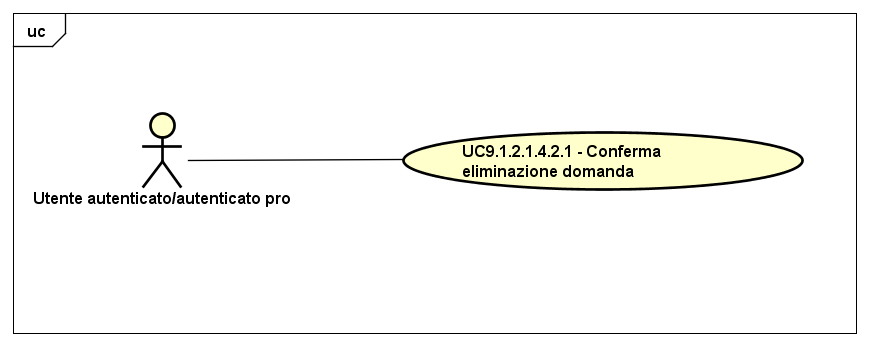
\includegraphics[scale=0.5,keepaspectratio]{UML/UC9_1_2_1_4_2.png}
							\caption{UC9.1.2.1.4.2: Elimina domande}
						\end{figure}
						\FloatBarrier
						\begin{itemize}
							\item \textbf{Attori}: \uau, \uaupro;
							\item \textbf{Descrizione}: l'utente può eliminare una domanda da un questionario;
							\item \textbf{Precondizione}: l'utente ha selezionato l'opzione "Elimina domanda" tra le scelte possibili in UC9.1.2.1.4;
							\item \textbf{Postcondizione}: l'utente ha eliminato una domanda;
							\item \textbf{Scenario principale}: l'utente deve confermare di voler eliminare la domanda (UC9.1.2.1.4.2.1); 
							\item \textbf{Scenari alternativi}: l'utente ha cancellato tutte le domande. Deve allora inserirne almeno una, viene allora rimandato a UC9.1.2.1.4.1.
						\end{itemize}
						
							\subsubsection{Caso d'uso UC9.1.2.1.4.2.1: Conferma eliminazione domanda}
							\label{UC9.1.2.1.4.2.1}
							\begin{itemize}
								\item \textbf{Attori}: \uau, \uaupro;
								\item \textbf{Descrizione}: l'utente deve confermare di voler eliminare la domanda;
								\item \textbf{Precondizione}: l'utente ha deciso di voler eliminare la domanda;
								\item \textbf{Postcondizione}: l'utente ha eliminato una domanda;
								\item \textbf{Scenario principale}: l'utente conferma di voler eliminare la domanda;
								\item \textbf{Scenari alternativi}: l'utente annulla l'eliminazione della domanda, viene allora rimandato a UC9.1.2.1.4.
							\end{itemize}	
																
					\subsubsection{Caso d'uso UC9.1.2.1.5: Conferma modifiche}
					\label{UC9.1.2.1.6}
					\begin{itemize}
						\item \textbf{Attori}: \uau, \uaupro;
						\item \textbf{Descrizione}: l'utente ha eseguito tutte le modifiche e ora deve salvare in modo che siano archiviate;
						\item \textbf{Precondizione}: l'utente ha selezionato l'opzione "Conferma modifiche" tra le scelte possibili in UC9.1.2.1;
						\item \textbf{Postcondizione}: l'utente ha confermato di volere salvare le modifiche fatte;
						\item \textbf{Scenario principale}: l'utente conferma di volere salvare le modifiche fatte;
						\item \textbf{Scenari alternativi}: l'utente non conferma e le modifiche fatte non vengono salvate. L'utente viene indirizzato alla pagina contenente la lista dei questionari da lui creati (UC9.1.2).
					\end{itemize}
										
			\subsubsection{Caso d'uso UC9.1.2.2: Elimina questionario}
			\label{UC9.1.2.2}
			\begin{figure}[h]
				\centering
			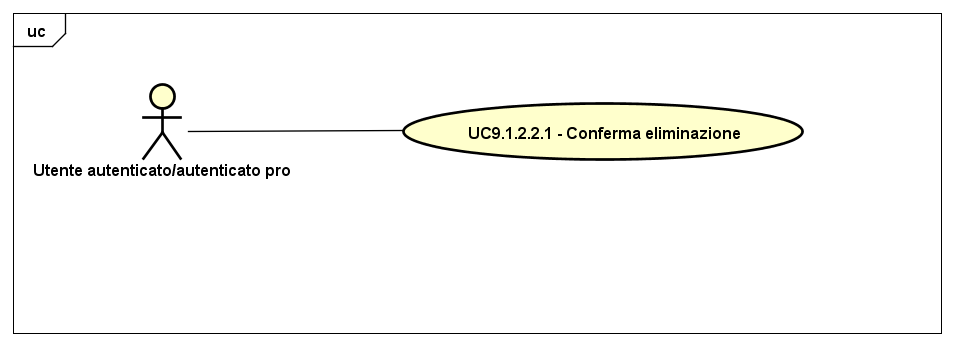
\includegraphics[scale=0.5,keepaspectratio]{UML/UC9_1_2_2.png}
				\caption{UC9.1.2.2: Elimina questionario}
			\end{figure}
			\FloatBarrier
			\begin{itemize}
				\item \textbf{Attori}: \uau, \uaupro;
				\item \textbf{Descrizione}: l'utente decide di voler eliminare il questionario dall'archivio di questionari;
				\item \textbf{Precondizione}: l'utente ha selezionato l'opzione "Elimina questionario" tra le scelte possibili in UC9.1.2;
				\item \textbf{Postcondizione}: l'utente ha eliminato il questionario;
				\item \textbf{Scenario principale}:l'utente deve confermare di voler eliminare il questionario (UC9.1.2.2.1);
			\end{itemize}
			
				\subsubsection{Caso d'uso UC9.1.2.2.1: Conferma eliminazione}
				\label{UC9.1.2.2.1}
				\begin{itemize}
					\item \textbf{Attori}: \uau, \uaupro;
					\item \textbf{Descrizione}: l'utente deve confermare di voler eliminare il questionario; 
					\item \textbf{Precondizione}: l'utente ha selezionato l'opzione "Conferma eliminazione" tra le scelte possibili in UC9.1.2.2;
					\item \textbf{Postcondizione}: l'utente ha confermato di voler eliminare il questionario;
					\item \textbf{Scenario principale}: l'utente conferma di voler eliminare il questionario;
					\item \textbf{Scenari alternativi}: l'utente non conferma di voler eliminare il questionario. L'utente viene indirizzato alla pagina contenente la lista dei questionari da lui creati (UC9.1.2).
				\end{itemize}
								
		\subsubsection{Caso d'uso UC9.1.3: Visualizza cronologia questionari svolti}
		\label{UC9.1.3}
		\begin{figure}[h]
			\centering
			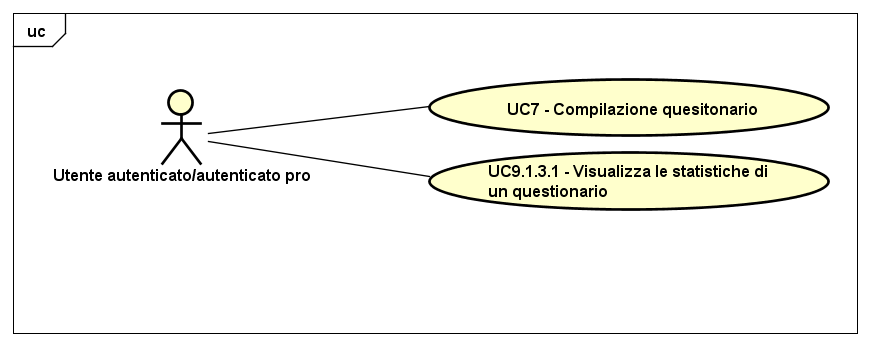
\includegraphics[scale=0.5,keepaspectratio]{UML/UC9_1_3.png}
			\caption{UC9.1.3: Visualizza cronologia questionari svolti}
		\end{figure}
		\FloatBarrier
		\begin{itemize}
			\item \textbf{Attori}: \uau, \uaupro;
			\item \textbf{Descrizione}: l'utente può visualizzare l'elenco dei questionari che ha svolto;
			\item \textbf{Precondizione}: l'utente ha selezionato l'opzione "Visualizza cronologia questionari svolti" tra le possibilità proposte in UC9.1;
			\item \textbf{Postcondizione}: il sistema ha eseguito le opzioni scelte dall'utente;
			\item \textbf{Scenario principale}: 
			\begin{enumerate}
				\item L'utente può compilare un questionario di nuovo (UC7);
				\item L'utente può visualizzare le statistiche di un questionario (UC9.1.3.1);
			\end{enumerate}
		\end{itemize}
		
				\subsubsection{Caso d'uso UC9.1.3.1: Visualizza le statistiche di un questionario}
				\label{UC9.1.3.1}
				\begin{itemize}
					\item \textbf{Attori}: \uau, \uaupro; 
					\item \textbf{Descrizione}: l'utente visualizza le statistiche di un questionario;
					\item \textbf{Precondizione}: l'utente ha scelto l'opzione "Visualizza le statistiche di un questionario" tra le scelte possibili in UC9.1.3;
					\item \textbf{Postcondizione}: l'utente ha visualizzato le statistiche di un questionario; 
					\item \textbf{Scenario principale}: l'utente visualizza le statistiche di un questionario;
				\end{itemize}
										
	\subsubsection{Caso d'uso UC9.2: Crea questionari}
	\label{UC9.2}
	\begin{figure}[h]
		\centering
	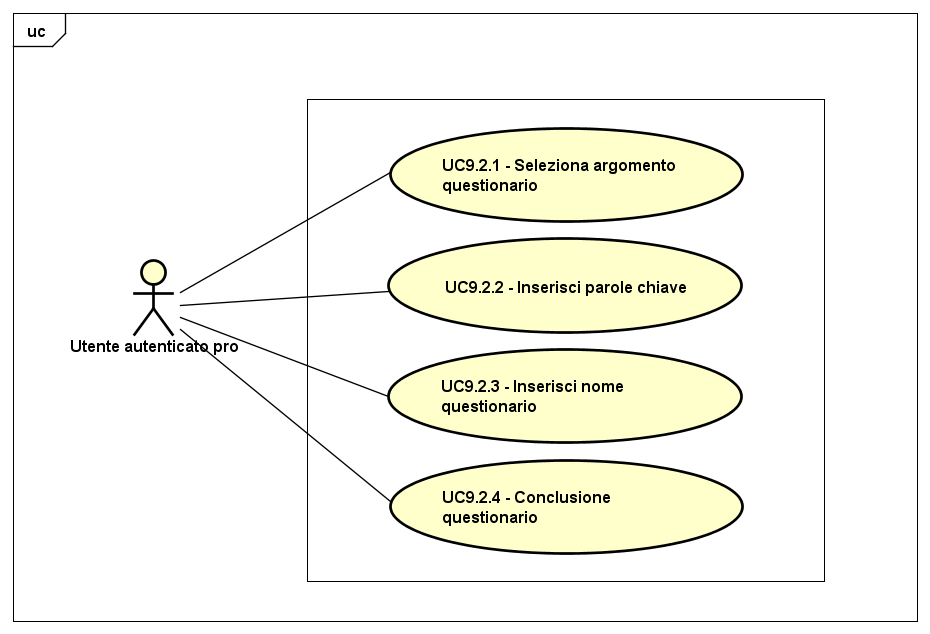
\includegraphics[scale=0.5,keepaspectratio]{UML/UC9_2.png}
		\caption{UC9.2: Crea questionari}
	\end{figure}
	\FloatBarrier
	\begin{itemize}
		\item \textbf{Attori}: \uau, \uaupro;
		\item \textbf{Descrizione}: l'utente può creare un nuovo questionario; 
		\item \textbf{Precondizione}: l'utente ha selezionato l'opzione "Crea questionari" tra le possibilità proposte in UC9;
		\item \textbf{Postcondizione}: l'utente ha creato un questionario;
		\item \textbf{Scenario principale}:
			\begin{enumerate}
				\item L'utente può selezionare la tipologia del questionario (UC9.2.1);
				\item L'utente può inserire il nome del questionario (UC9.2.2);
				\item L'utente può selezionare gli argomenti del questionario (UC9.2.3);
				\item L'utente può gestire le domande (UC9.2.4);
				\item L'utente può concludere il questionario (UC9.2.5);
			\end{enumerate}
	\end{itemize}
	
		\subsubsection{Caso d'uso UC9.2.1: Seleziona tipologia questionario}
		\label{UC9.2.1}
		\begin{itemize}
			\item \textbf{Attori}: \uau, \uaupro;
			\item \textbf{Descrizione}: l'utente può selezionare la tipologia del questionario; 
			\item \textbf{Precondizione}: l'utente ha selezionato l'opzione "Seleziona tipologia questionario" tra le scelte possibili in UC9.2;
			\item \textbf{Postcondizione}: l'utente ha selezionato la tipologia del questionario;
			\item \textbf{Scenario principale}: l'utente seleziona la tipologia del questionario;
			\item \textbf{Scenari alternativi}: l'utente non possiede un account pro e tenta di selezionare la tipologia privata per il questionario. Viene mandato in una pagina in cui può cambiare la tipologia del proprio account (UC5.7); 
		\end{itemize}
			
		\subsubsection{Caso d'uso UC9.2.2: Inserisci nome questionario}
		\label{UC9.2.2}
		\begin{itemize}
			\item \textbf{Attori}: \uau, \uaupro;
			\item \textbf{Descrizione}: l'utente può inserire il nome del questionario; 
			\item \textbf{Precondizione}: l'utente ha selezionato l'opzione "Inserisci nome questionario" tra le scelte possibili in UC9.2;
			\item \textbf{Postcondizione}: l'utente ha inserito il nome del questionario; 
			\item \textbf{Scenario principale}: l'utente inserisce il nome del questionario;
		\end{itemize}
		
		\subsubsection{Caso d'uso UC9.2.3: Seleziona argomenti questionario}
		\label{UC9.2.3}
		\begin{figure}[h]
			\centering
		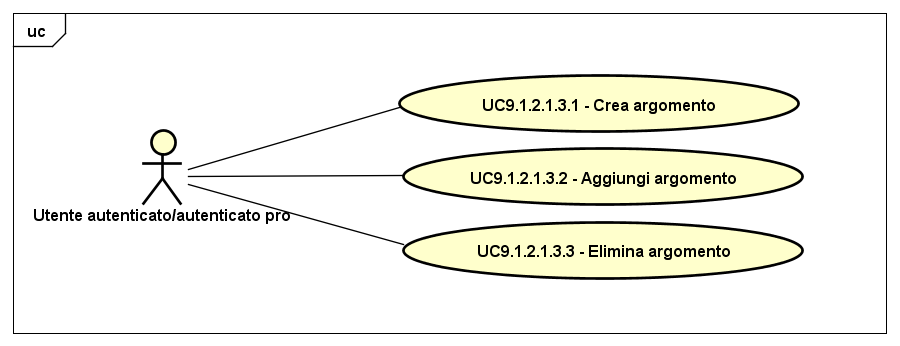
\includegraphics[scale=0.5,keepaspectratio]{UML/UC9_2_3.png}
			\caption{UC9.2.3: Seleziona argomenti questionario}
		\end{figure}
		\FloatBarrier
		\begin{itemize}
			\item \textbf{Attori}: \uau, \uaupro;
			\item \textbf{Descrizione}: l'utente può selezionare gli argomenti che riassumono il questionario;
			\item \textbf{Precondizione}: l'utente ha selezionato l'opzione "Seleziona argomenti questionario" tra le scelte possibili in UC9.2; 
			\item \textbf{Postcondizione}: l'utente ha selezionato gli argomenti che riassumono il questionario; 
			\item \textbf{Scenario principale}:
			\begin{enumerate}
				\item L'utente può creare un nuovo argomento (UC9.1.2.1.3.1);
				\item L'utente può aggiungere un nuovo argomento all'elenco di argomenti (UC9.1.2.1.3.2);
				\item L'utente può eliminare un argomento (UC9.1.2.1.3.3);
			\end{enumerate}
			\item \textbf{Scenari alternativi}: l'utente elimina tutti gli argomenti. In questo caso deve inserirne almeno uno e viene mandato al caso d'uso UC9.1.2.1.3.1.
		\end{itemize}
							
		\subsubsection{Caso d'uso UC9.2.4: Gestione domande}
		\label{UC9.2.4}
		\begin{figure}[h]
			\centering
			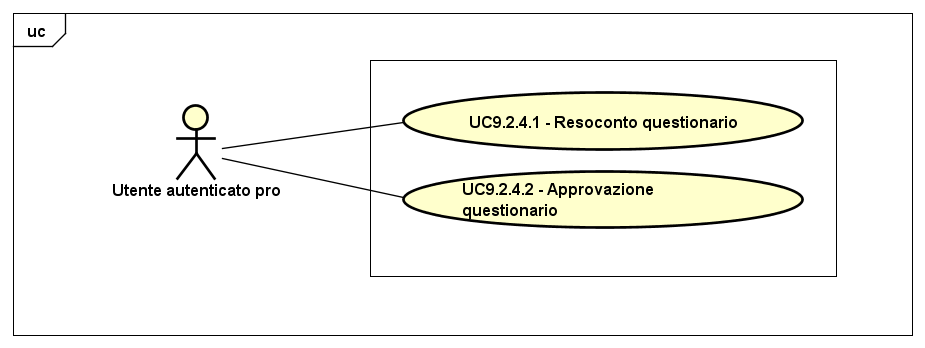
\includegraphics[scale=0.5,keepaspectratio]{UML/UC9_2_4.png}
			\caption{UC9.2.4: Gestione domande}
		\end{figure}
		\FloatBarrier
		\begin{itemize}
			\item \textbf{Attori}: \uau, \uaupro;
			\item \textbf{Descrizione}: l'utente può gestire le domande di un proprio questionario, aggiungendone oppure togliendone;
			\item \textbf{Precondizione}: l'utente ha selezionato l'opzione "Gestione domande" tra le scelte possibili in UC9.2;
			\item \textbf{Postcondizione}: l'utente ha gestito le domande di un questionario;
			\item \textbf{Scenario principale}: 
			\begin{enumerate}
				\item L'utente aggiunge altre domande (UC9.1.2.1.4.1);
				\item L'utente elimina una domanda (UC9.1.2.1.4.2).
			\end{enumerate}
		\end{itemize}
		
		\subsubsection{Caso d'uso UC9.2.5: Conclusione questionario}
		\label{UC9.2.5}
		\begin{figure}[h]
			\centering
			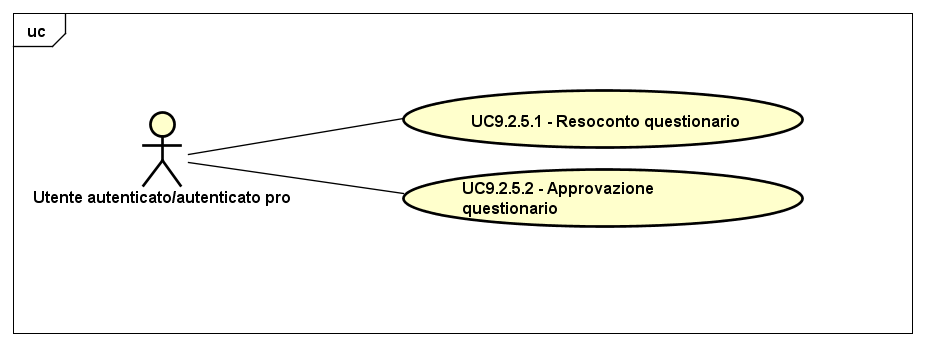
\includegraphics[scale=0.5,keepaspectratio]{UML/UC9_2_5.png}
			\caption{UC9.2.5: Conclusione questionario}
		\end{figure}
		\FloatBarrier
		\begin{itemize}
			\item \textbf{Attori}: \uau, \uaupro; 
			\item \textbf{Descrizione}: l'utente decide che il questionario è concluso;
			\item \textbf{Precondizione}: l'utente ha scelto l'opzione "Conclusione questionario" tra le scelte possibili in UC9.2;
			\item \textbf{Postcondizione}: l'utente ha completato il questionario;
			\item \textbf{Scenario principale}: 
				\begin{enumerate}
					\item L'utente visualizza il riepilogo finale del questionario appena creato (UC9.2.5.1); 
					\item L'utente approva la creazione del questionario (UC9.2.5.2); 
				\end{enumerate}
		\end{itemize}
				
			\subsubsection{Caso d'uso UC9.2.5.1: Resoconto questionario}
			\label{UC9.2.5.1}
			\begin{itemize}
				\item \textbf{Attori}: \uau, \uaupro;
				\item \textbf{Descrizione}: l'utente visualizza le scelte fatte finora per la creazione del questionario;
				\item \textbf{Precondizione}: l'utente ha scelto l'opzione "Resoconto questionario" tra le scelte possibili in UC9.2.5;
				\item \textbf{Postcondizione}: l'utente ha visualizzato le scelte fatte finora per la creazione del questionario;
				\item \textbf{Scenario principale}: l'utente visualizza le scelte fatte finora per la creazione del questionario;
			\end{itemize}
			
			\subsubsection{Caso d'uso UC9.2.5.2: Approvazione questionario}
			\label{UC9.2.5.2}
			\begin{itemize}
				\item \textbf{Attori}: \uau, \uaupro;
				\item \textbf{Descrizione}: l'utende deve approvare il questionario appena creato;
				\item \textbf{Precondizione}: l'utente ha scelto l'opzione "Approvazione questionario" tra le scelte possibili in UC9.2.5; 
				\item \textbf{Postcondizione}: l'utente ha approvato il questionario;
				\item \textbf{Scenario principale}: l'utente approva il questionario;
				\item \textbf{Scenari alternativi}: l'utente non approva il questionario e quest'ultimo non viene archiviato. L'utente viene mandato alla pagina precedente.
			\end{itemize}
	 
	
	